% =============================================================================
%  Section 2 -- Methodology
% =============================================================================

\section{Methodology}

% --- Section divider --------------------------------------------------------
\sectiondivider{Methodology}{From raw video to a 5-class quality score}{sec:methodology}

% --- Subsection: Pipeline ---------------------------------------------------
\subsection{Pipeline}

\begin{frame}{End-to-end pipeline}
\hypertarget{sub:pipeline}{}%
\centering
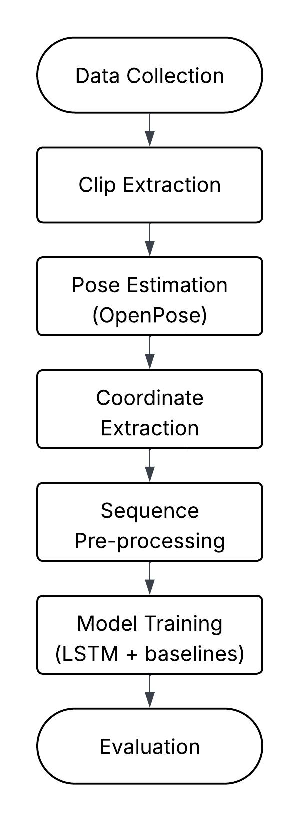
\includegraphics[width=0.92\linewidth,height=0.7\textheight,keepaspectratio]{./DATA/images/methodology/methodologyPipeline.pdf}\\[2pt]
{\scriptsize\itshape Seven modular stages, each independently inspectable and replaceable.}
\end{frame}

% --- Subsection: Data -------------------------------------------------------
\subsection{Data Collection \& Dataset}

\begin{frame}{Data collection \& labeling}
\hypertarget{sub:dataset}{}%
\begin{columns}[T,onlytextwidth]
\begin{column}{0.50\textwidth}
\textbf{\color{tecdark}Acquisition (controlled):}
\begin{itemize}\small
    \item iPhone 13, fixed \alert{vertical orientation}, 1080$\times$1920 HD @ 30 frames per second (FPS).
    \item 6 players, skill range: 6th category $\rightarrow$ professional.
    \item 484 clips, \alert{exactly 3\,s} each (90 frames @ 30\,\acrshort{FPS}).
\end{itemize}
\vspace{4pt}
\textbf{\color{tecdark}Labeling protocol:}
\begin{itemize}\small
    \item Each clip graded \alert{1--10} by a single expert coach.
    \item Grade embedded in filename (\texttt{\_grade}).
    \item Two evaluators: K.~Garc\'ia (CO), S.~Fasciolo (AR).
\end{itemize}
\end{column}
\begin{column}{0.48\textwidth}
\centering
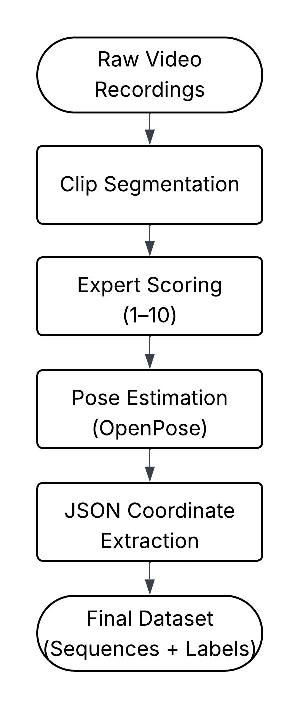
\includegraphics[width=\linewidth,height=0.68\textheight,keepaspectratio]{./DATA/images/methodology/dataCollection_Pipeline.pdf}\\[2pt]
{\scriptsize\itshape Six-stage data \& labeling workflow.}
\end{column}
\end{columns}
\end{frame}

\begin{frame}{Dataset \& 5-class mapping}
\begin{columns}[T,onlytextwidth]
\begin{column}{0.52\textwidth}
\small
Raw grades (1--10) $\rightarrow$ 5 quality classes:
\[
c = \min\!\bigl(\lfloor(y-1)/2\rfloor,\,4\bigr)
\]
\begin{center}\scriptsize
\begin{tabular}{lcc}
\toprule
\textbf{Class} & \textbf{Grades} & \textbf{N} \\
\midrule
Very Low  & 1--2  & 40  \\
Low       & 3--4  & 74  \\
Medium    & 5--6  & 132 \\
High      & 7--8  & 175 \\
Excellent & 9--10 & 63  \\
\midrule
\textbf{Total} & & \textbf{484} \\
\bottomrule
\end{tabular}
\end{center}
\vspace{2pt}
\begin{infoBox}\scriptsize
Skewed toward Medium / High $\rightarrow$ \alert{balanced class weights} in training.
\end{infoBox}
\end{column}
\begin{column}{0.46\textwidth}
\centering
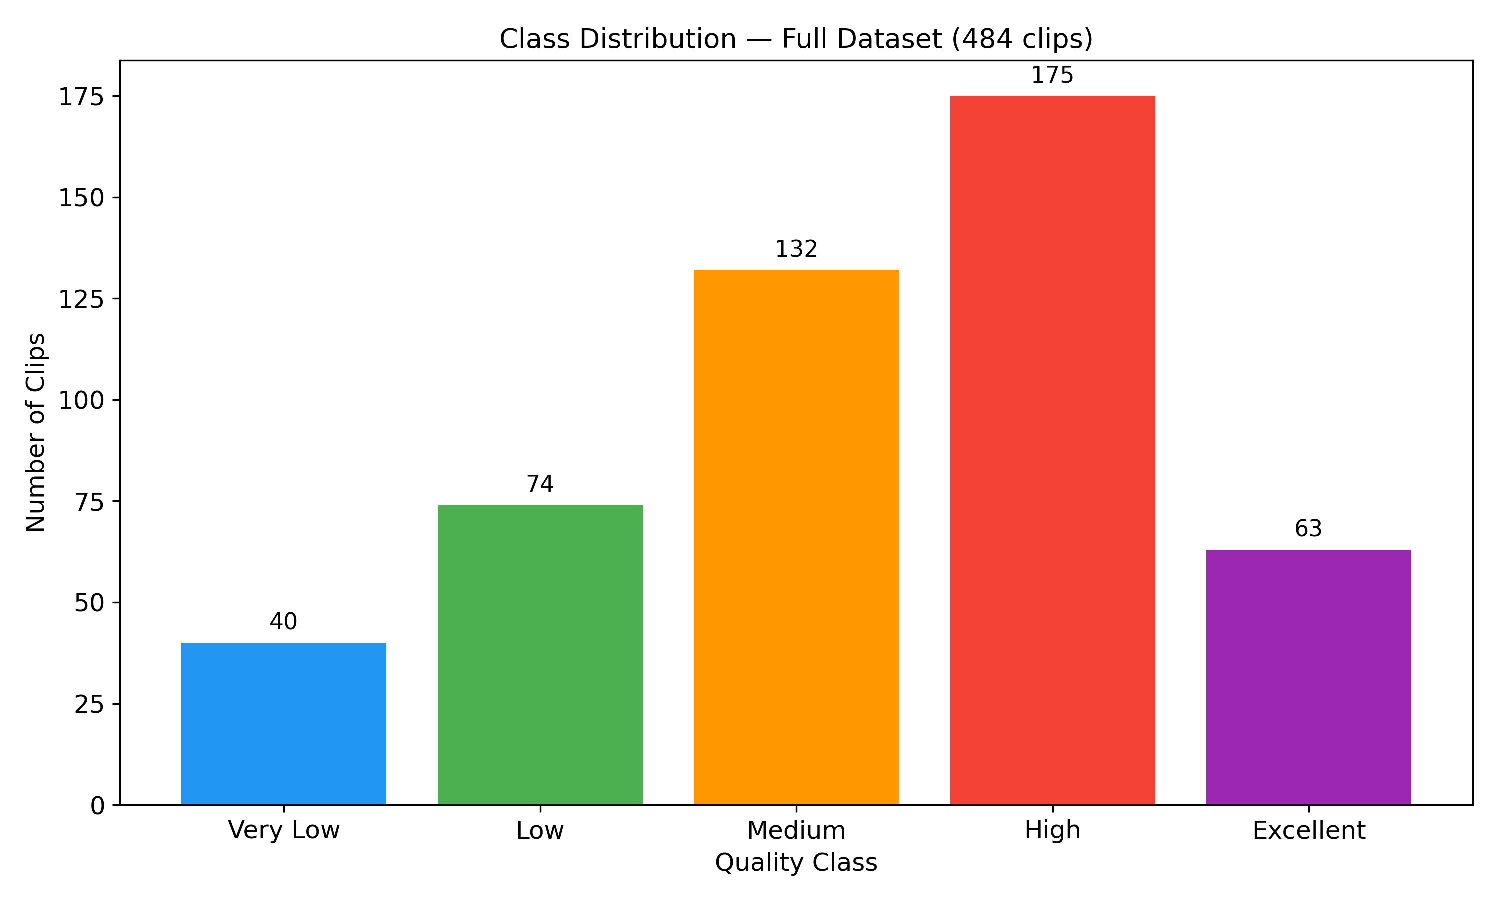
\includegraphics[width=\linewidth,height=0.62\textheight,keepaspectratio]{./DATA/images/experimentation/label_distribution.pdf}\\[2pt]
{\scriptsize\itshape Class distribution after the grade-to-class mapping.}
\end{column}
\end{columns}
\end{frame}

\begin{frame}{Dataset mosaic -- one frame per quality class}
\centering
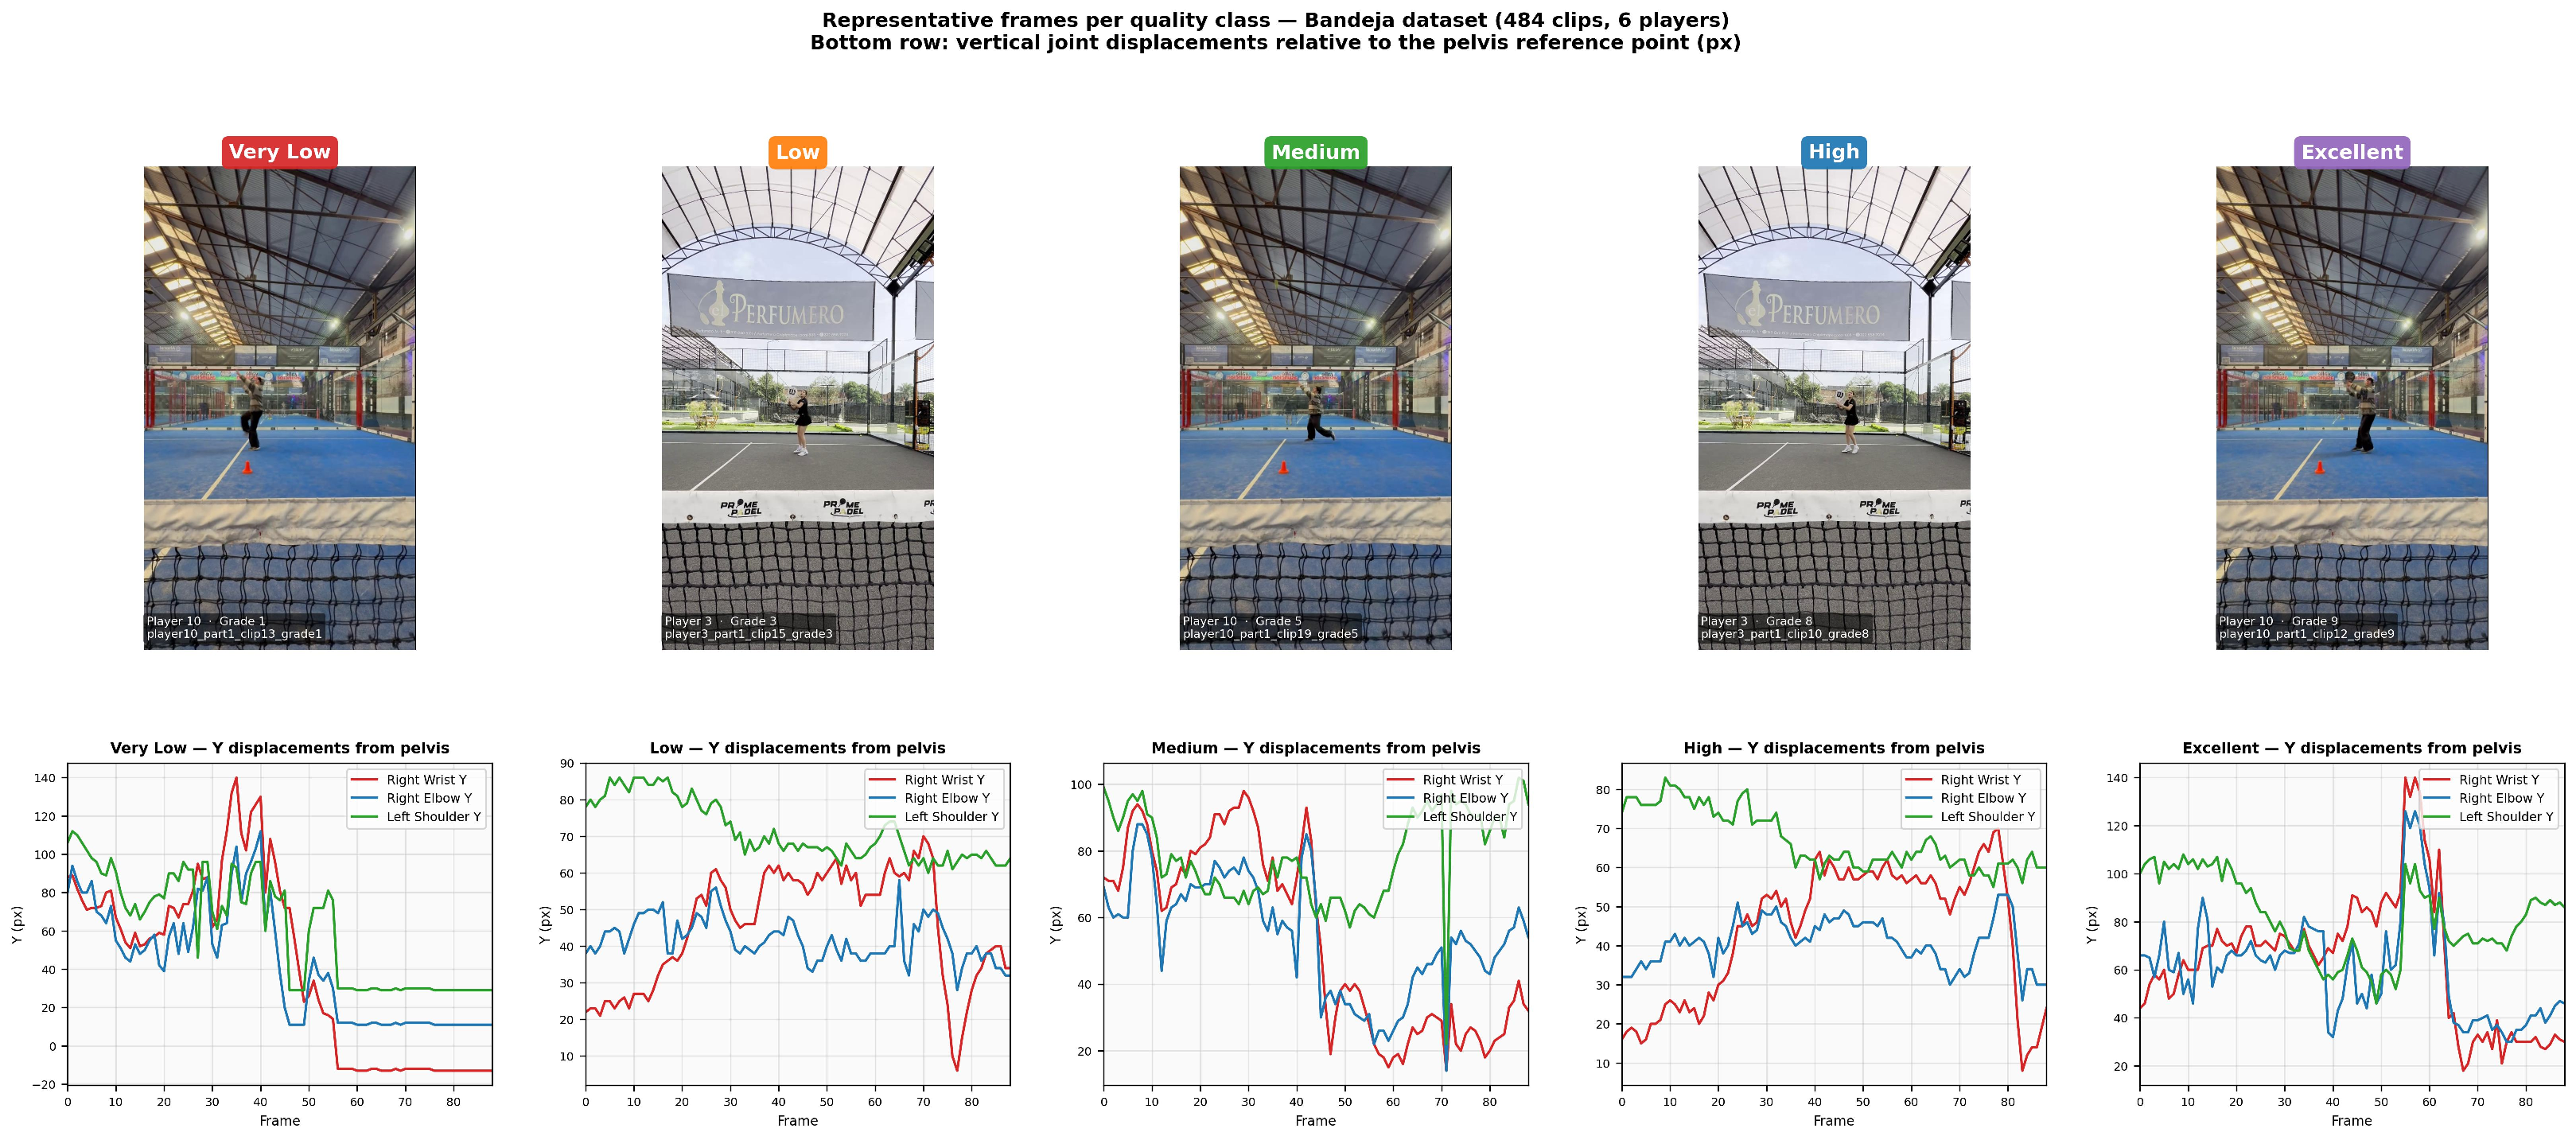
\includegraphics[width=\linewidth,height=0.66\textheight,keepaspectratio]{./DATA/images/experimentation/dataset_mosaic.pdf}\\[4pt]
{\footnotesize\textbf{\color{tecdark}Watch a representative clip:}}\\[1pt]
{\footnotesize
\setlength{\tabcolsep}{5pt}
\begin{tabular}{ccccc}
\href{https://github.com/CesarEmilioC/thesisRepo_A00830006/blob/main/Samples/mosaicSamples/player10_part1_clip13_grade1.mp4}{\textcolor{tecaccent}{\textbf{Very Low}}} &
\href{https://github.com/CesarEmilioC/thesisRepo_A00830006/blob/main/Samples/mosaicSamples/player3_part1_clip15_grade3.mp4}{\textcolor{tecorange}{\textbf{Low}}} &
\href{https://github.com/CesarEmilioC/thesisRepo_A00830006/blob/main/Samples/mosaicSamples/player10_part1_clip19_grade5.mp4}{\textcolor{tecblue}{\textbf{Medium}}} &
\href{https://github.com/CesarEmilioC/thesisRepo_A00830006/blob/main/Samples/mosaicSamples/player3_part1_clip10_grade8.mp4}{\textcolor{tecblue!70!tecgreen}{\textbf{High}}} &
\href{https://github.com/CesarEmilioC/thesisRepo_A00830006/blob/main/Samples/mosaicSamples/player10_part1_clip12_grade9.mp4}{\textcolor{tecgreen}{\textbf{Excellent}}}\\
{\scriptsize grades 1--2} & {\scriptsize grades 3--4} & {\scriptsize grades 5--6} & {\scriptsize grades 7--8} & {\scriptsize grades 9--10}\\
\end{tabular}
}\\[2pt]
{\scriptsize\itshape Click each class to open the corresponding clip on GitHub.}
\end{frame}

% --- Subsection: Pose features ---------------------------------------------
\subsection{Pose Features}

\begin{frame}{Pose estimation with OpenPose}
\hypertarget{sub:pose}{}%
\begin{columns}[T,onlytextwidth]
\begin{column}{0.52\textwidth}
\textbf{\color{tecdark}Joints retained (4)~\cite{Cao2019OpenPose}:}
\begin{itemize}\small
    \item \alert{Pelvis} -- positional reference (absolute).
    \item \alert{Left shoulder} -- trunk rotation.
    \item \alert{Right elbow} -- arm preparation.
    \item \alert{Right wrist} -- racket trajectory.
\end{itemize}
\vspace{4pt}
\textbf{\color{tecdark}Per clip $\Rightarrow$} sequence $\mathbf{X}_n\!\in\!\mathbb{R}^{F_n\times 8}$,\\
relative-to-pelvis $(x,y)$ for the 3 upper-body joints.
\vspace{4pt}
\begin{noteBox}\scriptsize
Linear interpolation fills missing detections.\\
Mean interpolation rate: \textbf{11.6\%} (consistent across classes).
\end{noteBox}
\end{column}
\begin{column}{0.46\textwidth}
\centering
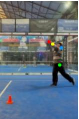
\includegraphics[width=\linewidth,height=0.65\textheight,keepaspectratio]{./DATA/images/methodology/poseEstimation_Example.pdf}\\[2pt]
{\scriptsize\itshape Pelvis (green), shoulder (blue), elbow (yellow), wrist (red)~\cite{Cao2019OpenPose}.}
\end{column}
\end{columns}
\end{frame}

\begin{frame}{What the model sees: \texttt{(90,\,8)} tensor of joint coordinates}
\hypertarget{sub:input}{}%
\begin{columns}[T,onlytextwidth]

% ---- LEFT: literal tensor preview ------------------------------------------
\begin{column}{0.54\textwidth}
\textbf{\color{tecdark}The literal input -- one tensor of shape \texttt{(90,\,8)} per clip:}\\[1pt]
{\scriptsize z-scored per clip $\cdot$ illustrative values $\cdot$ \textbf{720} numbers total}

\vspace{3pt}
\setlength{\tabcolsep}{2.5pt}
\renewcommand{\arraystretch}{1.02}
{\ttfamily\scriptsize
\begin{tabular}{r|rrrrrrrr}
\textbf{f} & \textbf{p$_x$} & \textbf{p$_y$} & \textbf{s$_x$} & \textbf{s$_y$} & \textbf{e$_x$} & \textbf{e$_y$} & \textbf{w$_x$} & \textbf{w$_y$}\\
\hline
0  & $-$1.20 & $-$0.85 & $-$0.42 &    0.13 & $-$0.78 &    0.24 & $-$1.05 &    0.31\\
1  & $-$1.15 & $-$0.81 & $-$0.38 &    0.17 & $-$0.70 &    0.30 & $-$0.95 &    0.40\\
2  & $-$1.10 & $-$0.78 & $-$0.34 &    0.21 & $-$0.62 &    0.36 & $-$0.85 &    0.49\\
\multicolumn{9}{c}{$\vdots$ \scriptsize (frames 3--43)}\\
44 &    0.05 & $-$0.12 &    0.28 &    0.95 &    0.55 &    1.62 &    1.10 &    2.18\\
45 &    0.07 & $-$0.10 &    0.31 &    0.98 &    0.58 &    1.65 &    1.13 &    2.21\\
\multicolumn{9}{c}{$\vdots$ \scriptsize (frames 46--88)}\\
89 &    0.85 &    0.42 &    0.71 &    0.18 &    1.08 &    0.55 &    0.92 &    0.81\\
\end{tabular}
}

\vspace{4pt}
{\scriptsize\textbf{Column legend:} \texttt{p}\,=\,pelvis (absolute), \texttt{s}\,=\,L-shoulder, \texttt{e}\,=\,R-elbow, \texttt{w}\,=\,R-wrist; subscripts $_x,_y$ = horizontal/vertical. The three upper-body joints are relative to the pelvis.}

\vspace{3pt}
\begin{infoBox}\scriptsize
\textbf{The model sees all 8 columns jointly} (pelvis + shoulder + elbow + wrist) -- not just one. The plot on the right visualises a single column for intuition.
\end{infoBox}
\end{column}

% ---- RIGHT: supporting trajectory plot ------------------------------------
\begin{column}{0.44\textwidth}
\centering
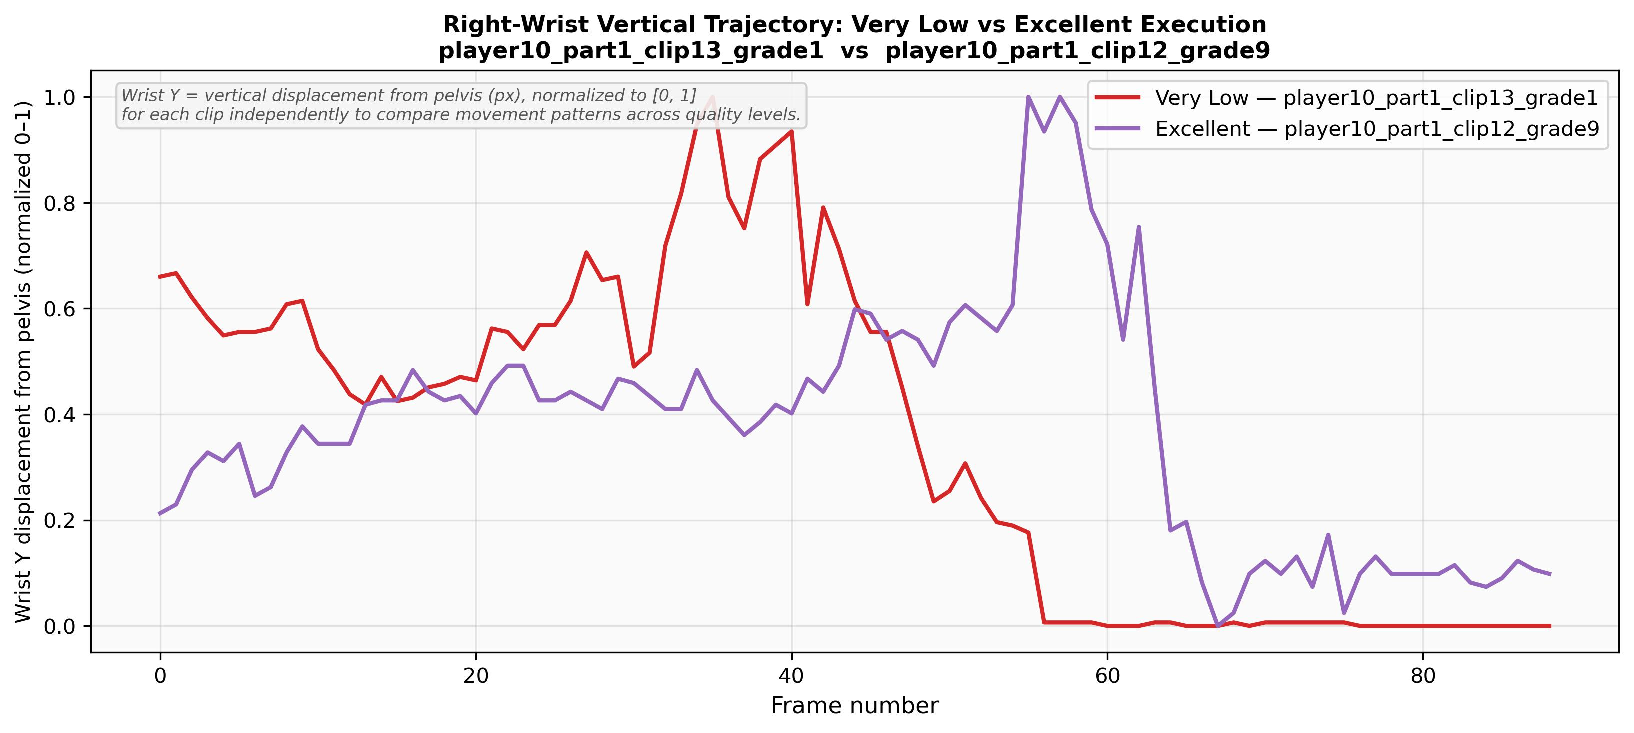
\includegraphics[width=\linewidth,height=0.56\textheight,keepaspectratio]{./DATA/images/methodology/trajectory_wrist_comparison.pdf}\\[2pt]
{\scriptsize\itshape \textbf{One of the 8 columns visualised:} the wrist trajectory across the 90 frames, for two clips of the same player. \alert{Excellent} (grade 9): smooth arc ($\sigma\!=\!40.1$~px). \alert{Very Low} (grade 1): irregular oscillations ($\sigma\!=\!184.1$~px). The remaining 7 columns evolve in parallel.}
\end{column}

\end{columns}
\end{frame}

% --- Subsection: Models -----------------------------------------------------
\subsection{Models}

\begin{frame}{Three temporal architectures}
\hypertarget{sub:models}{}%
\setlength{\tabcolsep}{4pt}
\small
\begin{center}
\begin{tabular}{l p{0.32\linewidth} p{0.36\linewidth}}
\toprule
\textbf{Model} & \textbf{Core block} & \textbf{Rationale} \\
\midrule
\textbf{BiLSTM}~\cite{Hochreiter1997LSTM} & 2 BiLSTM layers (64/32) + L2 weight decay + dropout 0.40/0.35 & 3-gate cell + cell state $\Rightarrow$ long-range memory \\
\addlinespace[2pt]
\textbf{BiGRU}~\cite{Cho2014GRU}  & 2 BiGRU layers (64/32) & 2-gate cell, fewer params (ablation) \\
\addlinespace[2pt]
\textbf{TCN}~\cite{Lea2017TCN}    & 3 dilated 1-D convs (kernel 3, dilation 1/2/4) + global average pooling (GAP) & Parallel processing, fixed receptive field \\
\bottomrule
\end{tabular}
\end{center}
\vspace{4pt}
\textbf{\color{tecdark}Shared training setup:}
\begin{itemize}\small
    \item Input $(90,8)$ $\rightarrow$ Softmax over 5 classes.
    \item Adam optimizer (Adaptive Moment estimation)~\cite{Adam2014}, sparse categorical cross-entropy, batch size 16, 100 epochs.
    \item EarlyStopping (patience 15), ReduceLROnPlateau, Gaussian noise augmentation (factor 2), \alert{balanced class weights}.
    \item 80/20 stratified split, seed 42.
\end{itemize}
\end{frame}

% --- Subsection: Evaluation -------------------------------------------------
\subsection{Evaluation Protocol}

\begin{frame}{Evaluation metrics -- categorical}
\hypertarget{sub:metrics}{}%
\small
For a $K$-class problem, with true positives ($\text{TP}_c$), false positives ($\text{FP}_c$), and false negatives ($\text{FN}_c$) per class $c$:
\vspace{4pt}
\begin{columns}[T,onlytextwidth]
\begin{column}{0.49\textwidth}
\begin{block}{Per-class\vphantom{Ag}}
\begin{minipage}[t][3.4cm][s]{\linewidth}
\centering\small
\vspace*{\fill}
$\displaystyle \text{Precision}_c = \frac{\text{TP}_c}{\text{TP}_c+\text{FP}_c}$\par
\vspace*{\fill}
$\displaystyle \text{Recall}_c = \frac{\text{TP}_c}{\text{TP}_c+\text{FN}_c}$\par
\vspace*{\fill}
$\displaystyle F_{1,c} = 2\cdot\frac{\text{Precision}_c \cdot \text{Recall}_c}{\text{Precision}_c + \text{Recall}_c}$\par
\vspace*{\fill}
\end{minipage}
\end{block}
\end{column}
\hspace{0.02\textwidth}
\begin{column}{0.49\textwidth}
\begin{block}{Aggregates\vphantom{Ag}}
\begin{minipage}[t][3.4cm][s]{\linewidth}
\centering\small
\vspace*{\fill}
$\displaystyle \text{Macro-}F_1 = \frac{1}{K}\sum_{c=1}^{K} F_{1,c}$\par
\vspace*{\fill}
$\displaystyle \text{Weighted-}F_1 = \sum_{c=1}^{K}\frac{n_c}{N}\,F_{1,c}$\par
\vspace*{\fill}
$\displaystyle \text{Accuracy} = \frac{\sum_c \text{TP}_c}{N}$\par
\vspace*{\fill}
\end{minipage}
\end{block}
\end{column}
\end{columns}
\vspace{4pt}
\begin{infoBox}\scriptsize
The \alert{confusion matrix} ($K\times K$) reveals \emph{where} errors land -- critical for ordinal tasks where adjacent-class confusion is expected but extreme-class confusion is not.
\end{infoBox}
\end{frame}

\begin{frame}{Evaluation metrics -- ordinal complement}
\begin{columns}[T,onlytextwidth]
\begin{column}{0.55\textwidth}
\small
The 5 quality classes carry a \alert{natural ordering}:
\[
\text{Very Low}\!<\!\text{Low}\!<\!\text{Medium}\!<\!\text{High}\!<\!\text{Excellent}
\]
Accuracy / F1 treat \emph{all} misclassifications as equally wrong. \alert{Spearman's $\rho$} captures monotonic agreement between predicted and true class rankings:
\[
\rho \;=\; \frac{\sum_i (R(y_i)\!-\!\overline{R(y)})\,(R(\hat{y}_i)\!-\!\overline{R(\hat{y})})}{\sqrt{\sum_i(R(y_i)\!-\!\overline{R(y)})^2 \sum_i(R(\hat{y}_i)\!-\!\overline{R(\hat{y})})^2}}
\]
\end{column}
\begin{column}{0.42\textwidth}
\begin{exampleblock}{Reading $\rho$}
\small
\begin{itemize}
    \item $\rho \!=\! +1$: perfect ordinal agreement.
    \item $\rho \!=\! 0$: no ordinal association.
    \item $\rho \!=\! -1$: perfect inverse ordering.
    \item Each $\rho$ paired with a $p$-value; \alert{$p\!<\!0.05$} required for statistical significance.
\end{itemize}
\end{exampleblock}
\vspace{4pt}
\begin{noteBox}\scriptsize
A high $\rho$ with modest accuracy means the model preserves the quality gradient even when the exact class is wrong.
\end{noteBox}
\end{column}
\end{columns}
\end{frame}
